The framework is illustrated in Fig. \ref{image:framework}, that also provides a key for reading this chapter. As shown, the semantics of our models is grounded on standard \emph{trace theory}~\cite{Hoare:1985}. A \emph{trace} is a finite sequence of symbols, a simple abstraction commonly used to capture the notion of ``observable behavior'' in the context of concurrent systems. In our case, the notion of behavior actually denotes interactions among agents forming a system. These interactions are modeled as \emph{events} sent and received by agents in a synchronous fashion. The (possibly infinite) set of traces that an agent or the system can exhibit, is captured with a kind of automata called labeled transition systems (LTS).

This trace-based setting is complemented with \emph{fluents}, that capture state-based propositions in terms of the occurrence of events. Among others, fluents provide a friendly interface between event-based models (e.g. scenarios and state machines) and state-based models (e.g. goals and domain properties). This mix of event-based and state-based abstractions provide a precise meaning, consistent \emph{semantics}, to all models used in this thesis. This semantics gives precise answers to questions like \emph{what traces does a scenario define?}, \emph{is this trace accepted by this state machine?}, \emph{does this sequence of events violate this safety goal?}, and so on.

\begin{figure}[t]\centering
  \scalebox{0.50}{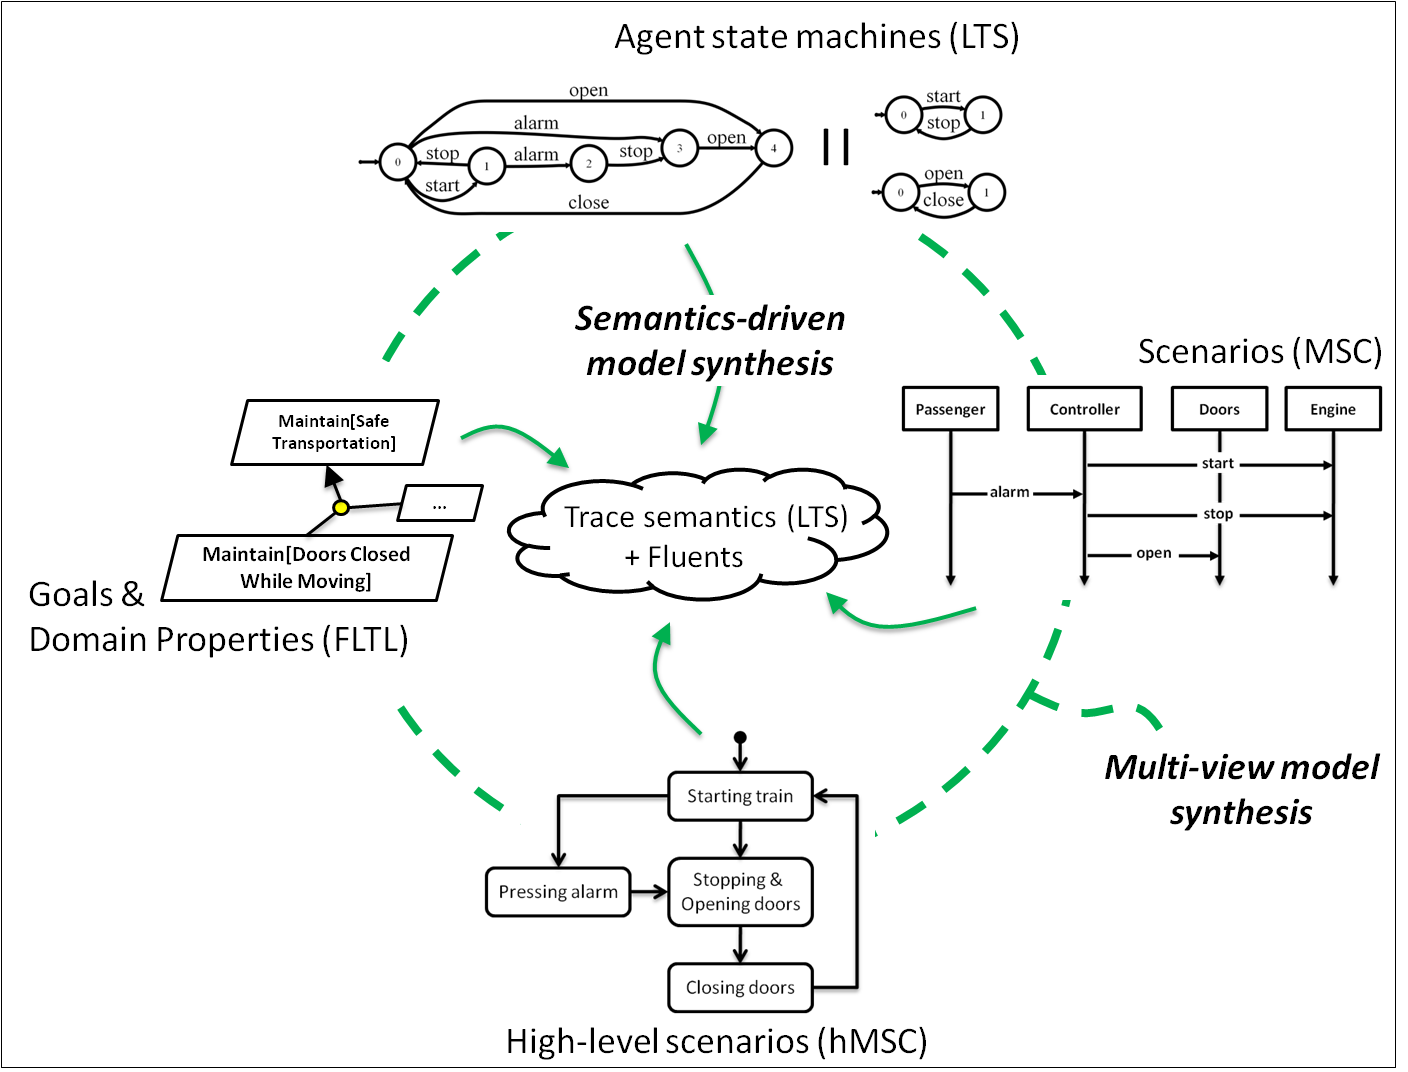
\includegraphics[trim=2mm 2mm 3mm 2mm, clip]{src/2-framework/images/framework}}
  \caption{Semantics and Multi-View consistency in our formal framework.\label{image:framework}}
\end{figure}

Observe however that LTSs are used in two different ways in this framework. On one hand, they provide a finite (and concrete) representation for infinite (and abstract) sets of traces used to define the semantics of other models. On the other hand, they are (not so) incidentally chosen as a particular representation for agent state machines (even if one could argue that such a representation is too low-level to be of any practical use for end-users). 

We stress this distinction here because, to our opinion, it explains the differences between two different, yet complementary, usages of model synthesis. In some approaches, so-called ``low-level models'' are used to define the semantics or help analyzing other, higher-level models. In this case, the former are used either theoretically as pure mathematical objects or, technically, as synthesized artifacts used as input for model checkers, animators, etc. Whatever the case, low-level models are commonly kept hidden to the end-user, in contrast to the higher-level ones which are used as input language for her (see, e.g.,~\cite{Magee:1997, Uchitel:2003, Damas:2009}). This contrasts with other approaches where different kinds of models are considered on an equal footing to form a consistent, multi-view representation of a system. In this second case, model synthesis aims at enriching the model basis by generating missing models, or completing existing ones. Therefore, synthesized models are visible to the end-user, who is expected to understand their intended meaning in a precise way (see, e.g.,~\cite{VanLamsweerde:1998, Whittle:2000, Uchitel:2004, Damas:2005}).

These two settings are of course complementary, so that the boundary is actually quite fuzzy. This is because providing automated support for a multi-view modeling approach requires formal models, which triggers for a mathematical characterization of their semantics and associated synthesis techniques (of the first kind). In contrast, because the trace semantics is actually very close to the state machines in the multi-view framework studied here, it might look like if the semantics of the other models was defined ``in terms of state machines''. This is, however, at best a shortcut and at worse a logical mistake.

This is of course not saying that scenarios and state machines (say) are not related in some way. In fact, in addition to the model semantics \emph{per se}, this chapter states rules governing their consistent usage for describing a given system. Such inter-model consistency rules are expressed in terms of the formal model semantics, but they are certainly not \emph{the same} as this semantics. In particular, they provide answers to another kind of questions than the aforementioned ones. Examples of such multi-view questions include \emph{is this scenario consistent with those agent state machines?}, \emph{is this safety goal violated by this system?}, \emph{is this scenario an implied one?} Observe that, in a sense, consistency rules give a fulcrum for both model synthesis and model checking (taken in a somewhat different, even broader, sense than usual). Indeed, model checking is applied \emph{against} them, that is, proving their respect or violation, while multi-view model synthesis is applied \emph{towards} them, by synthesizing missing models in a ``correct by construction'' fashion.


In addition to the notion of \emph{system}, that encompass all agents, the literature makes use of specific terms to distinguish between certain agents and/or agent aggregations. In~\cite{VanLamsweerde:2009} for example, the \emph{software-to-be} denotes software agent(s) that need to be developed (the automated controller, for example), while other agents compose its \emph{environment}. Another boundary consists in distinguishing the software together with its input and output devices from other agents. This boundary, depicted with a dashed line in Fig.~\ref{image:train-scenario-all-agents}, corresponds to the distinction made by Jackson between the \emph{world} and the \emph{machine}~\cite{Jackson:1995}. In this thesis, we focus on the behavior of a single agent as observed by the other agents with which it interacts (as opposed to its internal implementation). From the former agent perspective, then, the \emph{environment} is made of all these latter agents. 

In the light of the previous paragraph, we clearly need tools to capture single agent behaviors while being able to play with agent boundaries in a flexible manner -- for instance, for ``computing'' the behavior of agent aggregations like the \emph{software environment}, the \emph{machine} or simply, the \emph{system}. For this, we choose to model behaviors and interactions in an event-based framework, where agents communicate via messages that are sent and received simultaneously. Such kind of communication, called \emph{synchronous communication} or simply, \emph{message passing}, is motivated by its simplicity, an important aspect for accessibility to stakeholders involved during the early-design phase of a system. The next section introduces  labeled transition systems (LTS), the kind of model we use to capture agent behaviors. The next one presents operators for composing (and decomposing) them under a \emph{synchronous communication} hypothesis, a manner of capturing the behaviors of multiple interacting agents.


